\documentclass[12pt]{report}
\usepackage{graphicx}
\usepackage[utf8]{inputenc}
\usepackage[spanish]{babel}
\usepackage{setspace}
\usepackage{geometry}
\usepackage{titlesec}
\usepackage{times}
\usepackage{mathptmx} % Use mathptmx instead of times
\usepackage{fancyhdr}
\usepackage{float}
\usepackage{pdfpages}



% Configuración de márgenes
\geometry{
    top=2.5cm,
    left=3cm,
    right=3cm,
    bottom=2.5cm
}

% Configuración de interlineado
\onehalfspacing

% Configuración de títulos y subtítulos
\titleformat{\chapter}[display]
  {\normalfont\bfseries\centering}{}{0pt}{\fontsize{14}{16}\selectfont}
\titleformat{\section}
  {\normalfont\bfseries}{\thesection}{1em}{\fontsize{12}{14}\selectfont}
\titleformat{\subsection}
  {\normalfont\bfseries}{\thesubsection}{1em}{\fontsize{12}{14}\selectfont}


% Configuración de pie de página
  \fancyhf{}
\fancyfoot[R]{\thepage}
\pagestyle{fancy}
\fancypagestyle{plain}{
  \fancyhf{}
  \fancyfoot[R]{\thepage}
}

  \begin{document}
  \pagenumbering{roman}
%----- PORTADA ----
\setlength{\hoffset}{27 pt} % 1 (Para centrar más la portada)
\begin{titlepage}
{\centering
{\fontfamily{ptm}\scshape\bfseries\fontsize{29.16}{34.992}\selectfont Universidad de Guadalajara \par}
\vspace{0.5cm}
{\scshape\Large Centro Universitario de los Lagos \par}
\vspace{1cm}
{\scshape\Large División de Estudios de la Biodiversidad e innovación Tecnológica \par}
\vspace{1cm}
{\graphicspath{{imagenes/Portada}} %ruta de las imagenes

\includegraphics[width=0.3\textwidth]{image.png}\par}
\vspace{1cm}
% Título
{\scshape\large\bfseries Practica 6: Función temporizador (TON y TOF) \par}
\vspace{0.5cm}
% Materia
{\large \textbf{Materia:} \\Controladores Lógicos Programables\par}
\vfill
% Estudiante
{\large \textbf{Presenta:} \\Oscar Iván Moreno Gutiérrez \#220942754
\\Maximiliano Frias Campos \#217488066
\par}
\vfill
% Profesor
{\large \textbf{Profesor:} \\Dr. Afanador Delgado Samuel Mardoqueo \par}
\vfill
\vfill
% Fecha
\begin{flushright}
  {\normalsize \textbf {Fecha:} \\ \today}
\end{flushright}
\vfill}
{\large  \par}
\end{titlepage}
%----- FIN DE PORTADA ----

%----- ÍNDICE GENERAL ----
\tableofcontents
\newpage

%----- PALABRAS CLAVE ----
\pagenumbering{arabic}
\chapter*{Palabras Clave}
\begin{description}
  \item[Controladores Lógicos Programables (PLC):] Dispositivos utilizados para la automatización de procesos industriales mediante la programación de secuencias lógicas.
  \item[Temporizadores TON y TOF:] Funciones de temporización en PLCs que permiten controlar el tiempo de activación (TON) y desactivación (TOF) de una salida.
  \item[Simulación de circuitos de control:] Proceso de modelado y prueba de circuitos de control en un entorno virtual antes de su implementación física.
  \item[Retardo de activación y desactivación:] Tiempo específico que se introduce en un circuito para retrasar la activación o desactivación de una salida.
  \item[Programación de PLCs:] Proceso de escribir y cargar programas en un PLC para automatizar tareas específicas.
\end{description}
\addcontentsline{toc}{chapter}{Palabras Clave}


%\begin{itemize}

%\end{itemize}
\newpage

%----- OBJETIVO ----
\chapter*{Objetivo}
\addcontentsline{toc}{chapter}{Objetivo}
  El objetivo de esta Practica es utilizar los temporizadores de manera efectiva en la programación de Controladores Lógicos Programables (PLC) para controlar el tiempo de activación y desactivación de una salida. A través de la implementación de temporizadores TON y TOF, se busca simular y verificar el funcionamiento de circuitos de control que requieren un retardo específico para activar o desactivar una salida.

\newpage

%----- CONTENIDO ----
\chapter{Contenido}
\section{¿Qué es un temporizador?}
Un temporizador es un dispositivo que se utiliza para controlar el tiempo de activación y desactivación de una salida en un circuito de control. En la programación de Controladores Lógicos Programables (PLC), los temporizadores se utilizan para introducir retrasos específicos en la activación y desactivación de salidas, lo que permite controlar el tiempo de ejecución de una operación.
\subsection{Funcionamiento de TON}
La función TON (Temporizador ON Delay) se utiliza para activar una salida después de un retardo específico. Cuando se activa la condición de TON, la salida permanece en un estado bajo (apagado) durante un tiempo determinado antes de cambiar a un estado alto (encendido). Una vez que la salida se activa, permanece en ese estado durante un tiempo específico antes de volver a su estado inicial.
\subsection{Funcionamiento de TOF}
La función TOF (Temporizador OFF Delay) se utiliza para desactivar una salida después de un retardo específico. Cuando se activa la condición de TOF, la salida permanece en un estado alto (encendido) durante un tiempo determinado antes de cambiar a un estado bajo (apagado). Una vez que la salida se desactiva, permanece en ese estado durante un tiempo específico antes de volver a su estado inicial.


\section{Materiales}
Para la realización de esta práctica se utilizaron los siguientes materiales:

\begin{itemize}
  \item \textbf{Aplicación con picosoft:} Software utilizado para la simulación y programación de PLCs.
  \item \textbf{PLC:} Controlador Lógico Programable utilizado para la implementación del circuito.
  \item \textbf{Botonera:} Dispositivo que contiene los botones de arranque y paro.
  \item \textbf{Botones:} Componentes individuales de la botonera utilizados para controlar el circuito.
\end{itemize}

\section{Procedimiento}
\begin{enumerate}
  \item Declaramos las variables de nuestro circuito.
        \begin{figure}[H]
          \centering
          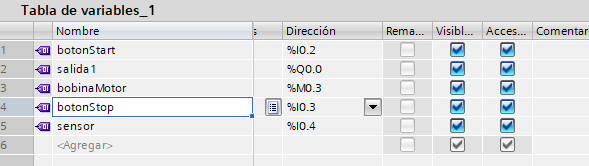
\includegraphics[width=0.5\textwidth]{screenshots/variables.png}
          \caption{Variables del circuito}
          \label{fig:variables}
        \end{figure}
  \item Creamos el circuito

\end{enumerate}
\newpage
\begin{figure}[H]
  \centering
  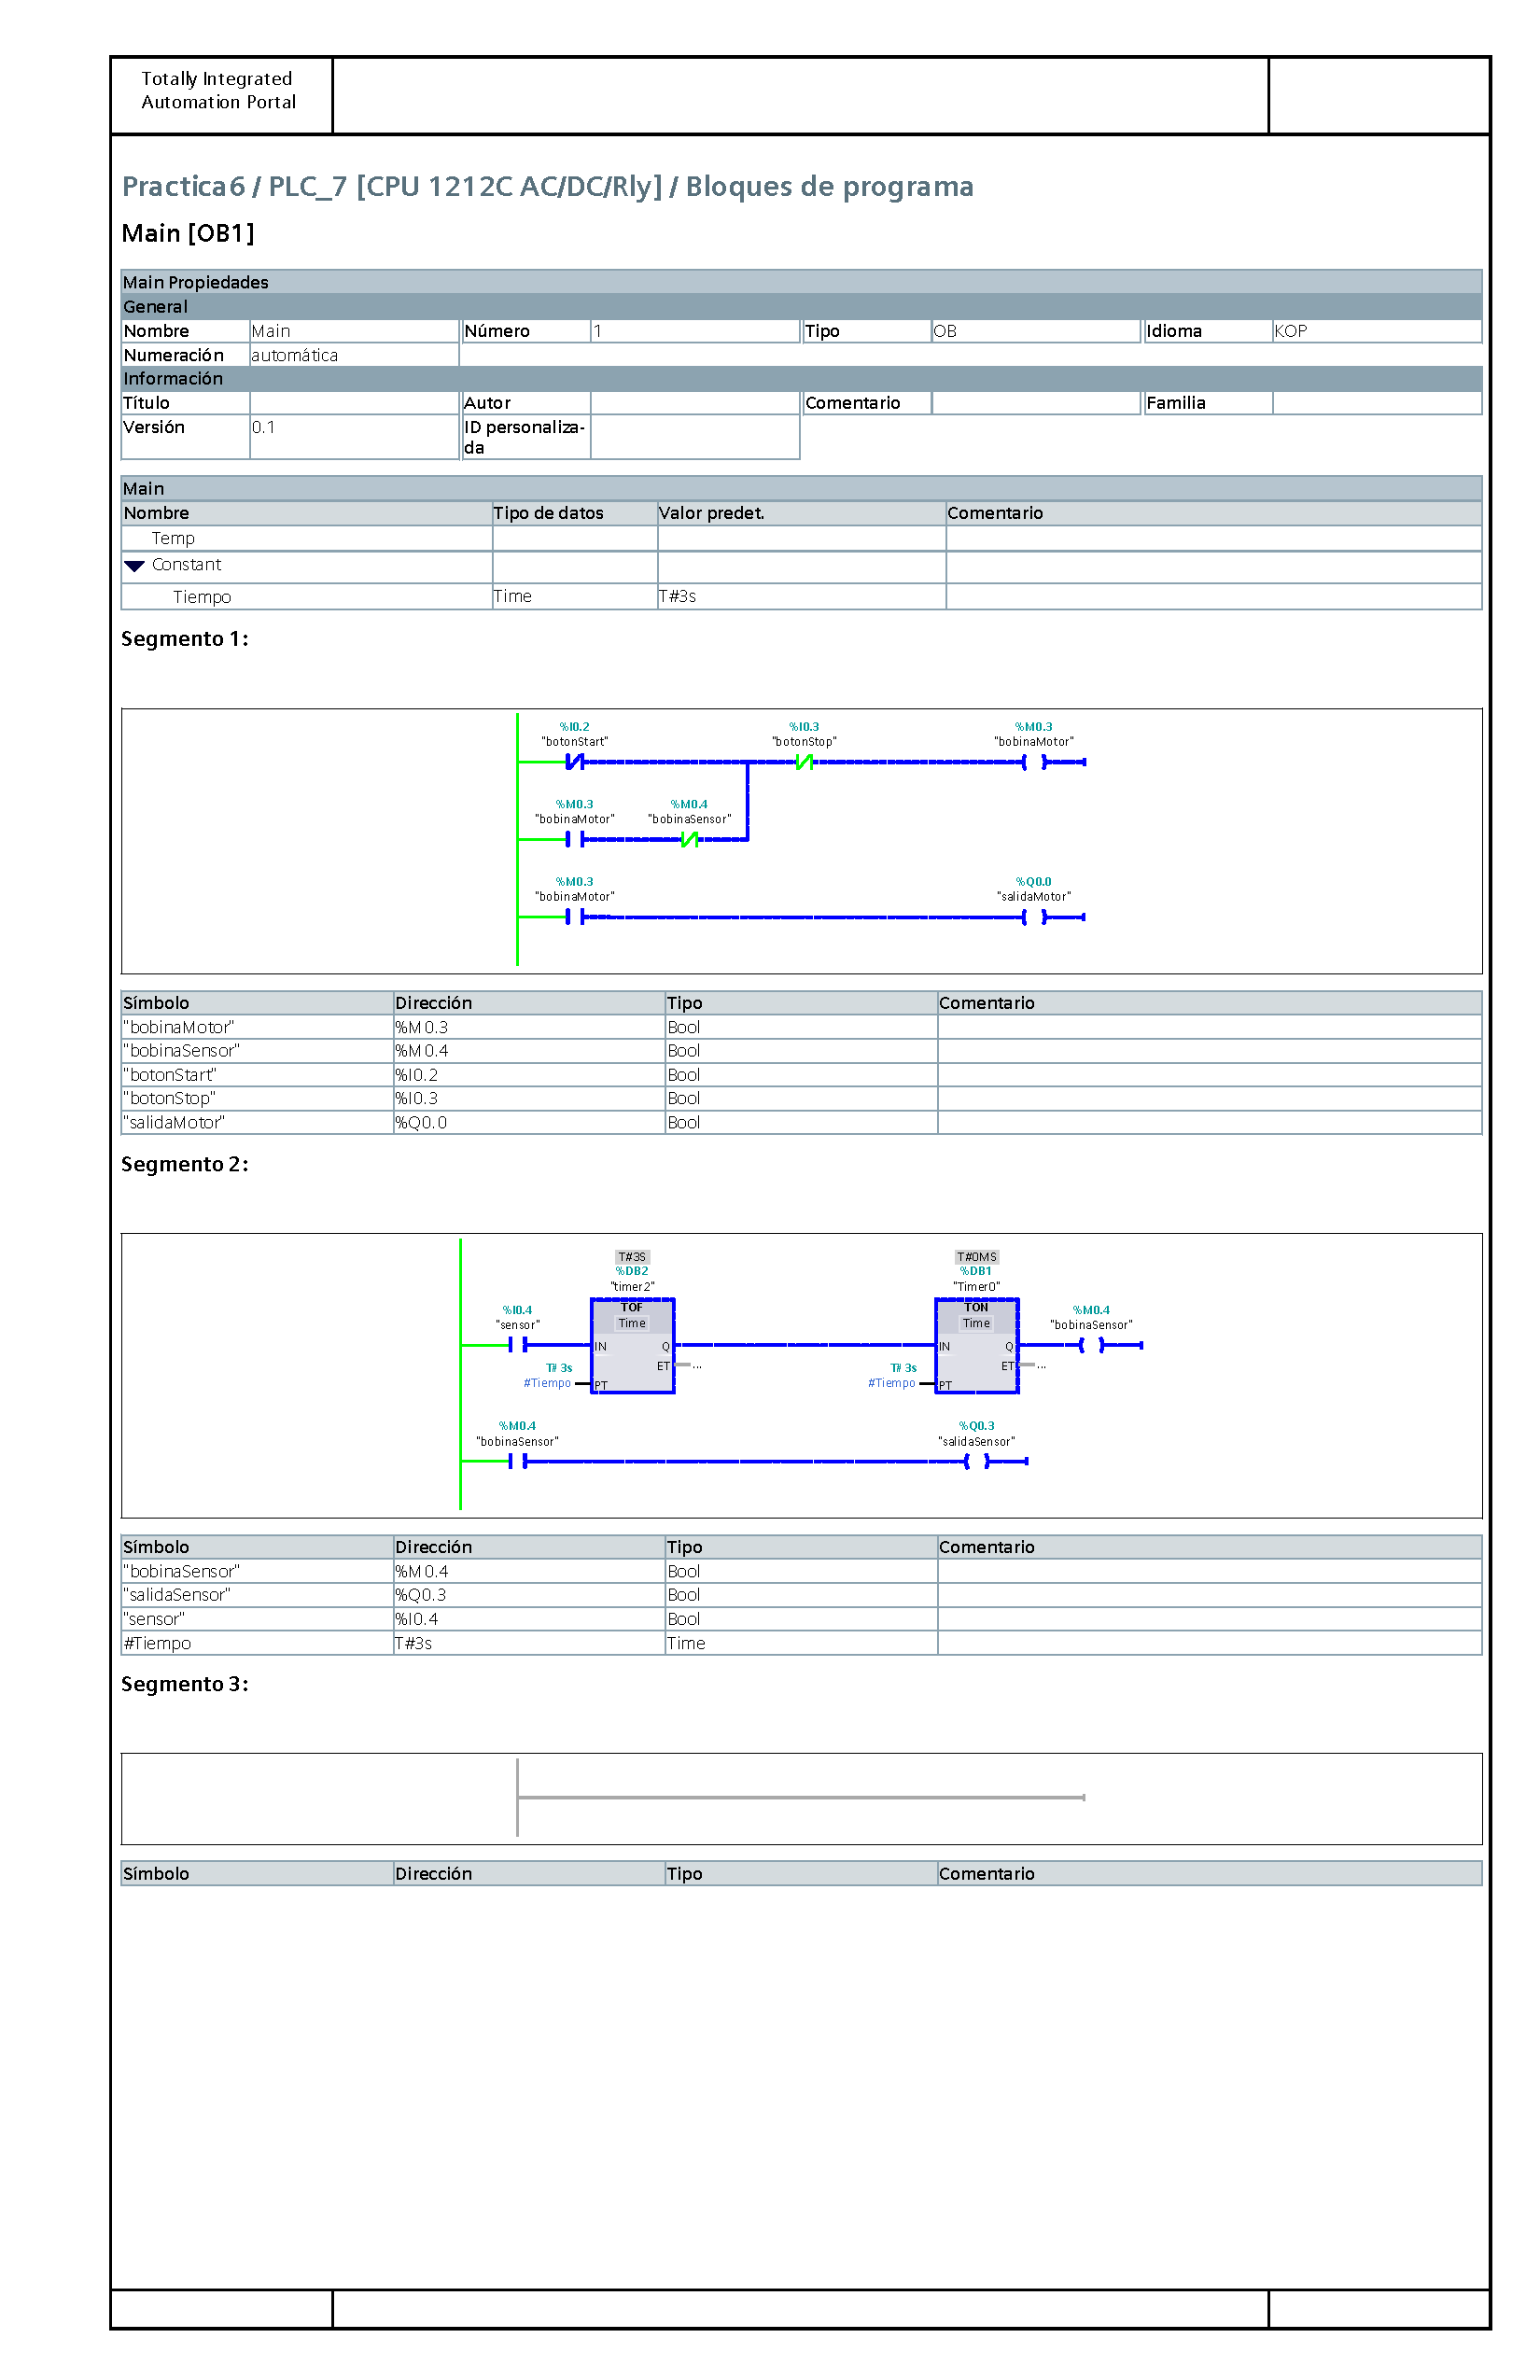
\includepdf[width=0.8\textwidth,page=1]{screenshots/p6.pdf} % Replace with the actual path to your PDF file
  \caption{circuito}
  \label{fig:pdfimage}
\end{figure}
\newpage

%----- CONCLUSIONES ----
\chapter{Conclusiones}
En esta práctica, aprendimos a utilizar los temporizadores TON y TOF en la programación de Controladores Lógicos Programables (PLC) para controlar el tiempo de activación y desactivación de una salida. A través de la implementación de temporizadores, pudimos simular y verificar el funcionamiento de circuitos de control que requieren un retardo específico para activar o desactivar una salida. Además, aprendimos a declarar variables y crear circuitos en el software de programación de PLCs, lo que nos permitió comprender mejor el proceso de programación y control de dispositivos electrónicos.
\newpage


\end{document}